\section{Sampling design}
\label{si:s2}

This section gives the full comparison of sampling schedules behind the two sampling rules of
the main text (sample across the dose cycle, never at the dose interval; record doses and intake
accurately), the conditions those rules rest on, and what each item of the routine record is
worth. Unless stated otherwise, every number is computed in the linear-clearance model at normal
capacity.

\subsection{Setting}
\label{si:s2:setting}

At each blood draw $i$ the marker $m_i$ (plasma 3-hydroxypropionate) is in quasi-steady state
(Section~\ref{si:s2:firsthour}), so the draw satisfies the balance of the linear-clearance model,
\begin{equation}
\label{seq:qss}
\bigl(\theta+\Delta(t_i)\bigr)\frac{m_i}{K_m+m_i}+k_e\,m_i \;=\; L_i+b ,
\end{equation}
where $\theta$ is the residual capacity (normal 3000\um), $\Delta(t)$ the enzyme delivered by the
infusions, $K_m$ the half-saturation constant of the enzymatic route, $k_e$ the rate constant of
the linear non-enzymatic route, $L_i$ the load recorded for that day and $b$ the unrecorded load
(the offset $L_0$ of the main text). The delivered increment is
$\Delta(t)=D\sum_{k:\,t_k\le t}e^{-\lambda(t-t_k)}$, with a dose jump $D=6000$\um\ (an assumed
value, which has not been measured) at infusions every $T=14$ days and $\lambda=\ln2/t_{1/2}$, $t_{1/2}=3.5$\,d. Therapy
starts at $t=0$, so the dose train is still accumulating over the first cycles; at steady state
the increment rises to 6400\um, $2.13\,\theta$, just after an infusion and falls to 400\um,
$0.133\,\theta$, at the trough (Supplementary Section~\ref{si:s1-eq}). The operating point is $K_m=100$\uM, $k_e=5$\,d$^{-1}$ and a baseline recorded load of
323\um, at which the marker moves between about 3 and 9\uM\ over the dose cycle. By the
\emph{phase} of a draw we mean its position in the dose cycle, the time since the last infusion.
% src: src/common/models.py:68-74; src/design/run.py:53-64; results/numbers/design.tex:50-51,115 (train_peak_frac 2.13); audit/brief_2026-10-01/out/t44_interval_decision.txt:4-5 (closed-form trough 400.0 = 0.133 x 3000, peak 6400.0; design.tex:117 prints 0.134 from the sampled train); manuscript/main.tex:593-603

The plasma assay carries a 5\% coefficient of variation and the recorded load a 5\% error;
combined in quadrature at the untreated operating level, they give an ordinate noise of
$\sigma=22.0$\um. Intake varies from day to day with a 10\%
coefficient of variation, and each draw is paired with the load recorded for its day. The
unknowns are $(\ln\theta,\ln K_m,b,\ln k_e)$. The prior on $k_e$ is log-normal with a standard
deviation of 0.8 on the log scale (a factor of 2.2), the prior on $b$ has a standard deviation of
5\% of the load, and no prior is placed on $\theta$ or $K_m$. Precision is the Cram\'er--Rao
bound from the Fisher information accumulated over the draws, reported as
$\sdl{\hat\theta}$, the standard deviation of the logarithm of the estimate, against the target
of 0.20. Unless stated otherwise, each value is a median over 24 simulated intake records of one
patient, with the range over records in brackets. A two-year record spans 730 days.
% src: src/design/run.py:44-45,115,185; results/numbers/design.tex:107; paper/sections/07_design.tex:39-67; manuscript/main.tex:682-703

$\sdl{\hat\theta}$ is a sampling spread. Read as an interval it is too narrow and too symmetric:
the 95\% profile-likelihood interval for $\theta$ on the monthly design spans a factor of 3.76
(median over 16 records; 2.86--5.08 across them), against the factor of 1.95 the bound implies,
with a long tail towards low $\theta$, because a lower capacity can be offset by a higher $K_m$.
% src: results/numbers/profile.tex:3-6; audit/brief_2026-10-01/out/n6_profile_vs_crb.txt:7-30; paper/sections/07_design.tex:214-233

\subsection{Why the infusions identify capacity}
\label{si:s2:excitation}

From Eq.~\eqref{seq:qss}, the sensitivities of a draw to $\ln K_m$ and to $\ln\theta$ stand in
the ratio
\begin{equation}
\label{seq:ratio}
\frac{\partial m/\partial\ln K_m}{\partial m/\partial\ln\theta}
\;=\;-\Bigl(1+\frac{\Delta(t)}{\theta}\Bigr)\,\varphi(m),
\qquad \varphi(m)=\frac{K_m}{K_m+m},
\end{equation}
so a record separates $\theta$ from $K_m$ only to the extent that this product changes from draw
to draw. It has two factors. The marker factor $\varphi(m)$ changes when the marker moves relative
to $K_m$; the dose factor $1+\Delta/\theta$ changes with the phase of the dose cycle. Over two
years of draws every two days at normal capacity and the baseline load, $\varphi$ runs from
0.9213 to 0.9675, a change
of 0.046, because the marker stays more than ten times below $K_m$. Over the same draws
$1+\Delta/\theta$ runs from 1.19 to 3.13, a change of 1.95 (a ratio of 2.64), and the product
changes by 1.94, 42 times the change in the marker factor alone.
% src: paper/sections/06_excitation.tex:125-137; results/tables/tab_D_factors.tex:5-7,9; results/numbers/design.tex:19,55,114,116; src/design/run.py:498-533

The same comparison can be put as a requirement. Taking as a reference an excitation of 0.50
(the change in $\varphi$ that a ninefold marker range centred on $K_m$ delivers; this is a
criterion we adopted, and the clinical question does not supply one), the marker route needs a
fold range
$r\ge\bigl((1+E)/(1-E)\bigr)^2$ placed about $K_m$, that is, a marker carried to many times its
managed level; the largest excursion a patient's record could contain, a decompensation to
eight times the operating level, reaches 0.35. The dose route instead needs
$(\Delta_{\max}-\Delta_{\min})/\theta\ge E/\varphi(\bar m)$, about 0.55 at the managed level,
and the fortnightly dose train supplies 1.95 on a schedule the protocol already fixes.
Supplementary Fig.~\ref{sfig:excitation} shows why the marker factor contributes so little.
% src: paper/sections/06_excitation.tex:139-152,182-196,198-216; results/numbers/design.tex:8,114

\begin{figure}[htbp]
\centering
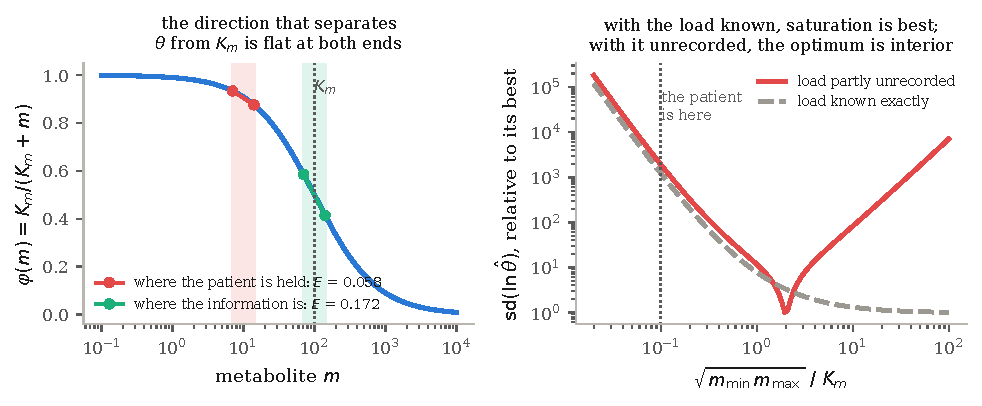
\includegraphics[width=\linewidth]{fig_D1_excitation.pdf}
\caption{\label{sfig:excitation}The marker factor of the excitation, in the linear-clearance
model ($K_m=100$\uM). Left: $\varphi(m)=K_m/(K_m+m)$, the factor through which the marker level
separates $\theta$ from $K_m$ (Eq.~\eqref{seq:ratio}), against the metabolite level $m$ (log
scale). It is flat far below and far above $K_m$ (dotted line), so what a set of draws
contributes is the drop in $\varphi$ across the levels it visits, its excitation $E$. The two
shaded bands span the same twofold range: centred on the managed level of 10\uM\ (red) they give
$E=0.058$; centred on $K_m$ (green) they give $E=0.172$. Right: the cost of placement in the
absence of therapy, as $\sdl{\hat\theta}$ for nine steady-state draws spread over a twofold band
of marker levels, each curve relative to its own best value, against the band's geometric centre
divided by $K_m$. Grey dashed, load known exactly: precision improves monotonically towards
saturation. Red, load partly unrecorded ($b$ estimated): the optimum is interior. The dotted
line marks the managed level, where precision is about 2\,100 times worse than at the optimum.
With the dose train it is the other factor, $1+\Delta/\theta$, that varies, so this limit does
not apply.}
% src: src/design/run.py:245-299; results/numbers/design.tex:3-4; paper/sections/06_excitation.tex:146-167
\end{figure}

\subsection{The schedules compared}
\label{si:s2:schedules}

Supplementary Table~\ref{stab:designs} compares the schedules on one footing. Therapy starts on
day 0 in every schedule; the draws start on the same day and run for two years, except that the
one-cycle schedule covers only the first dose cycle and the six-monthly visits fall at 180, 360,
540 and 720 days. Panel (b) repeats four of the schedules at an equal number of visits. The precision follows the range of $\Delta/\theta$ the draws see more closely than the
number of draws. Thirteen two-monthly draws reach the target (0.188), and 53 draws at the dose
interval miss it by a factor of 23 (4.58). Six-monthly visits see a range of 0.45 and miss it
(0.457). Seven draws
over one dose cycle see almost the whole range (1.81) but reach only 0.216, a limit set by the
design itself rather than by how well the increment is known. The correlation between
$\ln\hat\theta$ and $\ln\hat K_m$ tracks the same quantity, from $+0.999$ at the dose interval to
$+0.03$ for draws every two days.
% src: results/tables/tab_D_designs.tex:5-11; results/numbers/design.tex:10-16,56-58,91-104; src/design/run.py:1307-1317 (schedule times); paper/sections/07_design.tex:109-123,254-268

Booking every 14.5 days for two years (51 visits) gives 0.1615, the precision of monthly draws at
fortnightly density. At an equal 25 visits the three schedules that move through the cycle
(every 14.5 days, monthly and phase-spread) agree to within 3\% (0.170--0.174), but they take
different calendar time: the 14.5-day schedule needs 348 days, the monthly and phase-spread
schedules about two years. A phase-spread schedule books each
visit at a chosen phase so that the phases are spread evenly over the cycle, with visits at
least a month apart.
% src: results/numbers/design.tex:52,59-61,108; results/numbers/phaseclock.tex:22-26; audit/PHASE3_DESIGN.md:38-41; audit/g_design_common.py:40-80

The last row of panel (a) is given for reference only. The same 365 draws placed to straddle
$K_m$ (marker levels of 50--200\uM) would give 0.0157, 9.5 times better than the routine
placement, but they require holding the marker an order of magnitude above the 3--10\uM\ a
managed patient visits.
% src: results/tables/tab_D_designs.tex:11; results/numbers/design.tex:99-101,109; paper/sections/07_design.tex:254-260

\begin{table}[htbp]
\centering\small\setlength{\tabcolsep}{4.5pt}
\caption{\label{stab:designs}Precision of each sampling schedule on residual capacity, in the
linear-clearance model at normal capacity ($\theta=3000$\um), with the assumed dose ($D=6000$\um\
every 14 days, half-life 3.5\,d) starting on day 0, the day of the first draw (six-monthly:
visits at 180--720 days; one dose cycle: days 0--12). $n$, number of draws; levels
visited, the range of marker levels (\textmu M) the draws see; range of $\Delta/\theta$, the
spread of the delivered increment over the draws, relative to capacity; corr, posterior
correlation of $\ln\hat\theta$ with $\ln\hat K_m$. $\theta$ and $K_m$ are free; $k_e$ carries a
log-normal prior with standard deviation 0.8 on the log scale, the unrecorded load a prior of
5\% of the load; intake varies 10\% from day to day and is recorded to 5\%. (a)~Two-year records,
medians over 24 intake records with the range in brackets. (b)~25 visits each, medians over 8
intake records; span is the calendar time the 25 visits take. --, not computed.}
\begin{tabular}{@{}lrlccr@{}}
\toprule
\multicolumn{6}{@{}l}{(a) two-year record}\\
\midrule
schedule & $n$ & levels visited & range of $\Delta/\theta$ & $\sdl{\hat\theta}$ & corr \\
\midrule
at the dose interval, every 14\,d & 53 & 2.39--4.53 & 0.13 & 4.58 [3.51, 5.64] & $+0.999$ \\
every 14.5\,d & 51 & -- & 1.99 & 0.1615 [0.1611, 0.1618] & -- \\
monthly, every 30.4\,d & 25 & 2.81--9.47 & 1.84 & 0.1699 [0.1684, 0.1709] & $+0.336$ \\
two-monthly, every 60\,d & 13 & 3.28--9.70 & 1.94 & 0.1876 [0.1839, 0.1939] & $+0.471$ \\
every 2\,d & 365 & 2.49--10.47 & 1.95 & 0.1500 [0.1498, 0.1501] & $+0.033$ \\
one dose cycle, every 2\,d & 7 & 3.28--7.79 & 1.81 & 0.2162 [0.2053, 0.2300] & $+0.614$ \\
six-monthly & 4 & 5.76--10.34 & 0.45 & 0.457 [0.412, 0.510] & $+0.928$ \\
\emph{reference: 365 draws straddling $K_m$} & 365 & 50--200 & 1.95 & 0.0157 & $+0.206$ \\
\midrule
\multicolumn{6}{@{}l}{(b) 25 visits}\\
\midrule
schedule & $n$ & span (days) & range of $\Delta/\theta$ & $\sdl{\hat\theta}$ & \\
\midrule
at the dose interval, every 14\,d & 25 & 336 & 0.13 & 4.78 [3.51, 5.47] & \\
every 14.5\,d & 25 & 348 & 1.80 & 0.1739 [0.1732, 0.1757] & \\
monthly, every 30.4\,d & 25 & 730 & 1.84 & 0.1698 [0.1688, 0.1709] & \\
phase-spread & 25 & 738 & 1.85 & 0.1707 [0.1698, 0.1723] & \\
\bottomrule
\end{tabular}
% src: results/tables/tab_D_designs.tex:5-11,14; results/numbers/design.tex:13,52,59-61; results/numbers/phaseclock.tex:13-16,22-27; results/numbers/lattice.tex:38; audit/PHASE3_DESIGN.md:38-41; src/design/run.py:775-777,1308-1316,1499
\end{table}

\subsection{Aliasing at the dose interval, and the lap rule}
\label{si:s2:aliasing}

Draws booked at the dose interval, or at a multiple of it, all fall at one phase. The range of
$\Delta/\theta$ they see collapses from the monthly design's 1.84 to 0.13, and even that 0.13 is
only the dose train filling during the first cycles after therapy starts: for a patient already on
therapy the range is exactly zero, and at a constant recorded load the design is exactly singular
(Supplementary Fig.~\ref{sfig:conditioning}c). From therapy start, $\sdl{\hat\theta}$ goes to 4.58
(3.51--5.64), 27 times less precise than monthly draws, record by record 21--33 times. The same
aliasing costs a factor of 20--25 on the precision of $K_m$.
% src: results/numbers/design.tex:5-7,10,12,56-58; audit/PHASE3_DESIGN.md:60-65,312-327; paper/sections/07_design.tex:177-185,238-243

Write the booking interval as $h=kT+\epsilon$, where $kT$ is the nearest multiple of the dose
interval $T$ and $\epsilon$ the offset from it. When $\epsilon$ is small compared with $T$, each
visit falls $\epsilon$ later in the cycle than the last, so $n$ visits sweep $n\epsilon$ of it,
and the draws have covered the whole cycle once when
\begin{equation}
\label{seq:lap}
n\,\epsilon\;\ge\;T
\end{equation}
(the lap rule). For 14.5-day bookings $\epsilon=0.5$\,d, so 28 visits make one lap; the 51 visits
of a two-year record make 1.8 laps and 25 visits make 89\% of one. Monthly bookings ($h=30.4$\,d,
$k=2$, $\epsilon=2.4$\,d) sweep 4.3 laps in 25 visits. Over a two-year record of 53 visits the
rule needs $\epsilon\ge6.3$\,h. When $\epsilon$ is not small compared with $T$, successive draws
jump around the cycle instead of sweeping it, and coverage has to be checked directly, which the
phase-spread schedule does by construction.
% src: results/numbers/phaseclock.tex:8-12; results/numbers/lattice.tex:11,16,18,19; results/numbers/design.tex:48,52; paper/sections/07_design.tex:125-140; manuscript/main.tex:705-711
Supplementary Fig.~\ref{sfig:phaseclock} draws these coverage patterns for 25 visits of each
schedule.

\begin{figure}[htbp]
\centering
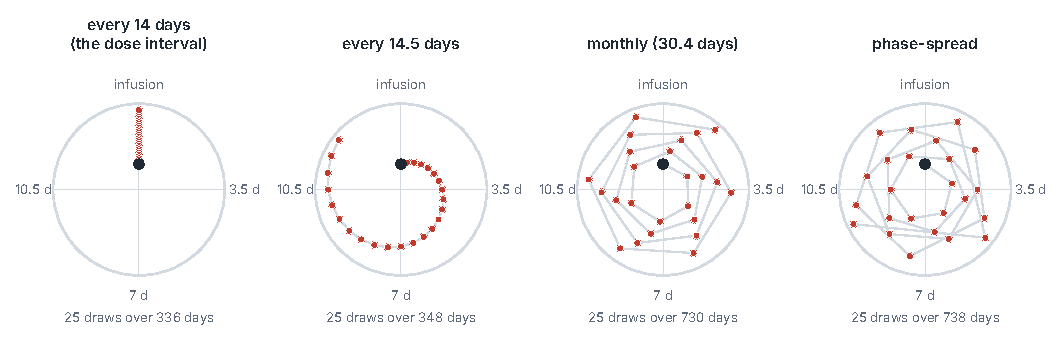
\includegraphics[width=\linewidth]{fig_S_phaseclock.pdf}
\caption{\label{sfig:phaseclock}Where the blood draws of each schedule fall in the 14-day dose
cycle. Each dot is one draw, placed around the circle by the number of days since the last
infusion (infusion at the top, time running clockwise) and outward by visit number (first visit
innermost, black dot). Twenty-five draws per schedule, starting on the day of the first infusion,
as in main-text Fig.~2b. Draws every 14 days all fall at the infusion and stack on one ray. Draws
every 14.5 days fall half a day later at each visit and wind round 89\% of the cycle. Monthly
draws, each 2.4 days later in the cycle than the last, and phase-spread draws, aimed at evenly
spaced points of the cycle, cover all of it. Draw times are those of the analysis code
(\texttt{audit/g\_design\_common.py}).}
\end{figure}

The rule marks where the cost of incomplete coverage stops falling, and below it the cost rises
gradually. Holding $n$
fixed and comparing each schedule with one that laps, the cost is a factor of 8.6 at 4\% of a lap,
3.4 at 10\%, 1.6 at 25\%, 1.1 at 50\% and 1.0 at 75\%. For a short record the lap matters more
than the number of visits: at the 14.5-day step, 20 visits instead of 25 sweep 71\% of a lap
instead of 89\% and cost a factor of 1.09, of which 1.06 is the incomplete lap and only 1.03 the
five missing visits. Booking every 14.7 days instead, so that 20 visits complete a lap
($\epsilon\ge16.8$\,h), takes the same 20 visits from 0.190 to 0.176, within about 1\% of 25 visits
at 14.5 days.
% src: results/numbers/lattice.tex:3-10,12,15-16,24,27,36-38; paper/sections/07_design.tex:142-175

Avoiding multiples of the dose interval is not sufficient. Booking every 14.01 days avoids every
multiple and reaches 53 distinct phases in two years, more than any other schedule here, but they
are packed into 12.5 hours of the 14-day cycle because $n\epsilon$ falls far short of a lap, and
the design gives 1.46. A protocol should therefore state the coverage requirement,
Eq.~\eqref{seq:lap}, and not only the prohibition.
% src: results/numbers/lattice.tex:29-33; paper/sections/07_design.tex:196-204

\subsection{How many visits}
\label{si:s2:visits}

Supplementary Fig.~\ref{sfig:visits} gives the precision against the number of visits. On the
footing of this section (prior on $k_e$ 0.8, intake varying 10\% from day to day; medians over 8
intake records), the monthly
schedule reaches the target at 11 visits and the phase-spread schedule at 10. The 14.5-day
schedule needs 20, because its early visits have not yet covered the cycle, and the dose-interval
schedule never reaches it. Once a schedule has covered the cycle, its curve follows
$\sdl{\hat\theta}=\sqrt{f^2+c^2/n}$, where $f$ is a floor that further visits cannot remove. On
the monthly schedule $f=0.150$ and $c=0.39$; at the dose interval $f=4.5$. The floor is set by the
prior on $k_e$ rather than by the visits: for monthly draws it falls from 0.150 at a prior of 0.8 to
0.059 at 0.3, 0.020 at 0.05 and 0.018 with $k_e$ known, while $c$ stays at about 0.39, and
tightening the prior from 0.8 to 0.3 brings the target from 11 visits to 6. About a dozen
well-placed visits therefore suffice; once the curve reaches its floor, further precision would
come from the prior rather than from the data.
% src: audit/PHASE3_DESIGN.md:82-98; paper/sections/07_design.tex:441-457,476-482

\begin{figure}[htbp]
\centering
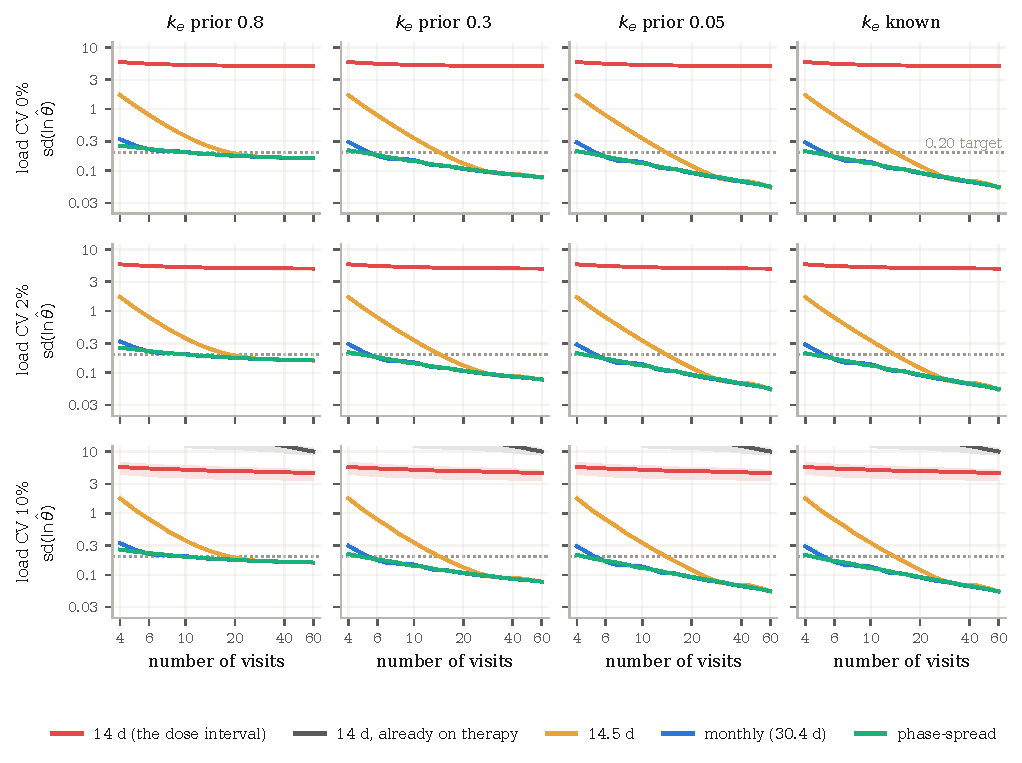
\includegraphics[width=0.86\linewidth]{fig_E2_visits.pdf}
\caption{\label{sfig:visits}Precision against the number of visits, in the linear-clearance model
at normal capacity. Each curve is $\sdl{\hat\theta}$ (log scale) against the number of visits
(log scale) for one schedule: at the 14-day dose interval from the start of therapy (red), at the
dose interval for a patient already on therapy (dark grey), every 14.5 days (orange), monthly
(blue) and phase-spread (green). The dark grey schedule is exactly singular at a constant load
and lies above the plotted range at 2\% variation; at 10\% its median stays above 10 up to 60
visits, so it shows only at the top of the bottom row. Columns: the standard deviation of
the log-normal prior on $k_e$ (0.8, the value used throughout, 0.3 and 0.05) and $k_e$ known.
Rows: day-to-day variation of intake (coefficient of variation 0, 2 and 10\%, labelled load CV).
Dotted line, the target of 0.20. Medians over 8 intake records; at 10\% variation the shading
gives the range. All curves assume the 5\% prior on the unrecorded load and an exactly known dose
scale; the near identity of the three rows reflects that prior rather than the design
(Supplementary Fig.~\ref{sfig:conditioning}a).}
% src: audit/PHASE3_DESIGN.md:66-98,122-130; paper/sections/07_design.tex:441-457; audit/g2_visits_vs_sd.py:96-120 (plot limits 0.02--12); dark grey medians recomputed with audit/g_design_common.py, 8 records (2%: 45--199; 10%: 10.0--46.6 over 4--60 visits)
\end{figure}

Supplementary Fig.~\ref{sfig:conditioning} releases, one at a time, three conditions behind those
curves. (a)~Without the prior on the unrecorded load, a constant recorded load makes every
schedule exactly singular at any number of visits; with 2\% day-to-day variation the monthly
schedule gives 0.348 at 12 visits and does not reach the target within 60, and with 10\% it gives
0.198 and reaches it at 12. (b)~If the dose scale is uncertain, at the 11.7\% the target
requires on these 8 records (11.6\% over 24 records, Section~\ref{si:s2:record}) the monthly
schedule needs about 30 visits instead of 11, and
at 20\% it does not reach the target within 60. (c)~For a patient already on therapy, draws at the
dose interval see no variation at all: exactly singular at a constant load, 20.8 (11.3--36.3)
at 12 visits with 10\% variation. The schedules that move through the cycle are unchanged by the
start time (monthly 0.189 from the start of therapy against 0.188 on therapy, at 12 visits and a
constant load).
% src: audit/PHASE3_DESIGN.md:250-262,280-292,312-330; paper/sections/A1_supplementary.tex:355-365

\begin{figure}[htbp]
\centering
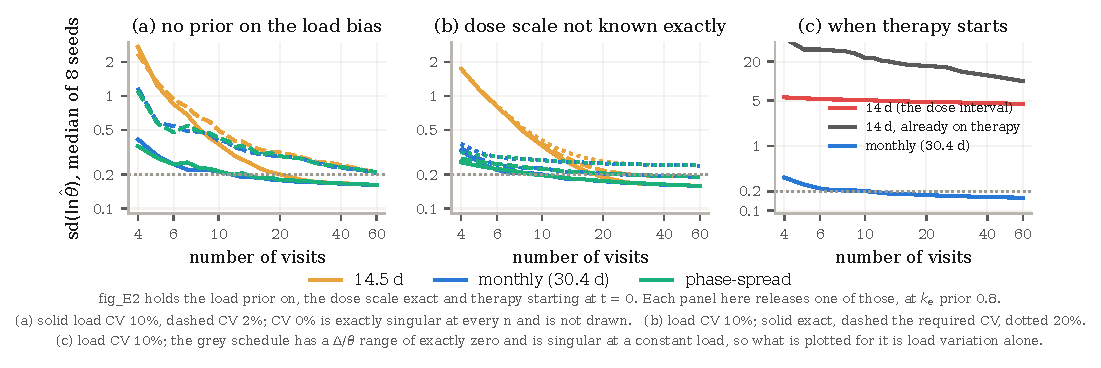
\includegraphics[width=\linewidth]{fig_E4_conditioning.pdf}
\caption{\label{sfig:conditioning}What the curves of Supplementary Fig.~\ref{sfig:visits} are
conditional on. Each panel gives $\sdl{\hat\theta}$ against the number of visits (log scales,
prior on $k_e$ 0.8, medians over 8 intake records; dotted line, target 0.20) with one condition
released. (a)~No prior on the unrecorded load: solid, intake varying 10\% from day to day;
dashed, 2\%; a perfectly steady recorded load is exactly singular at every number of visits and
is not drawn. (b)~Dose scale not known exactly, at 10\% intake variation: solid, exact; dashed,
known to 11.7\%, the requirement as solved over the 8 records of this figure (11.6\% over 24
records, Supplementary Table~\ref{stab:requirements}); dotted, 20\%. (c)~When therapy starts, at
10\% intake variation: draws at the 14-day dose interval from the start of therapy (red), at the
dose interval when the patient is already on therapy (dark grey; at a constant load this
schedule is exactly singular), and monthly draws (blue). In (a) and (b), orange, every 14.5 days;
blue, monthly; green, phase-spread. The ranking of schedules is the same under all three
conditions, but the absolute precisions change.}
% src: paper/sections/A1_supplementary.tex:352-366; audit/PHASE3_DESIGN.md:236-330; audit/g5_conditions.py:111-142
\end{figure}

Because the dose interval is exactly two weeks, each phase falls on a fixed weekday as long as
infusions are given exactly 14 days apart at a fixed time of day. For a weekday clinic, of 27
half-day phases outside
the infusion slot, 19 can be booked whatever the time of the infusion; with a morning infusion
the trough falls at a weekend and 96\% of the increment range remains reachable, with an
afternoon infusion the whole range is. Moving monthly visits to the nearest weekday costs about
2\% in precision (0.189 to 0.193 at 12 visits); without the move, a third of monthly visits would
fall at a weekend. A 12-visit phase-spread calendar on clinic days, with an afternoon infusion,
gives 0.193 (0.189--0.196) with the dose known exactly, but 0.220 at the dose-scale requirement, where the same construction
needs 36 visits. The calendar should be re-derived from the actual infusion dates, since a moved
infusion moves every later phase.
% src: audit/PHASE3_DESIGN.md:134-150,156-163,210-233,296-306; paper/sections/07_design.tex:459-473; results/figures/fig_E3_calendar.pdf (not reproduced)


\subsection{What the record must carry}
\label{si:s2:record}

Supplementary Table~\ref{stab:requirements} collects the requirements on the record. The
requirements on the delivered increment and on $k_e$ were solved for, holding the rest of the
design fixed, as the precision of that one quantity at which 25 monthly draws reach exactly 0.20;
the accuracy of the intake record is given as a sweep.
% src: paper/sections/08_specification.tex:38-45; results/tables/tab_D_loadprec.tex

\paragraph{The dosing record and the delivered increment.} The date, dose and lot of every
infusion enter the analysis as the known input $\Delta(t)$. Their value rests on how well the
amount each infusion delivers is known. If the delivered increment is known only up to a common
scale factor with a prior coefficient of variation $c_\Delta$, the monthly design reaches the
target at $c_\Delta=11.6\%$ (11.4--11.9\% across records), and the two-monthly design needs
7.7\% (5.3--8.7\%). The prior on the scale does not tighten as the record lengthens, so each
$c_\Delta$ carries a floor that no number of visits removes; the floor crosses the target at
about 18.7\%. The only published repeatability of a measurement that could supply the increment,
the 1-$^{13}$C-propionate breath test, is between visits two months to four years apart in 15
patients with methylmalonic acidaemia: a coefficient of variation of 14.0\% on average
($\pm12.9\%$, range 0.4--50.8\%)~\cite{breath_test_mma}. At 14.0\% the monthly design gives 0.212
after two years and reaches the target only after 118 monthly draws (9.8 years), against 11 with
the increment known exactly. A same-day pair of tests around one dose would need a coefficient of
variation 1.21 times lower (a 17\% reduction) than the between-visit figure, which bounds same-day error from
above because it includes drift between visits. The per-patient range (to 50.8\%) means that a
cohort meeting the requirement on average could still include patients for whom no record
suffices.
% src: results/numbers/design.tex:35-40; results/numbers/tier1.tex:3-13; paper/sections/08_specification.tex:118-169; paper/claims.csv:44

\paragraph{The dose calibration.} The assumed dose was chosen so that the marker falls by about
two thirds at the peak of the delivered enzyme (66\% at the steady-state peak; 62--66\%
depending on the baseline and the peak from which the fall is read). The interim report of the trial gives
smaller mean falls in 3-hydroxypropionate, at most 29\% in any dose cohort~\cite{trial_phase12},
and it does not state when after a dose the marker was sampled. Supplementary
Table~\ref{stab:dosesens} recomputes the design with the dose recalibrated to a 20\% or 30\% fall,
read either at the peak or at the trough, and at a half-life of 3.5 days (the assumed design
value) or 7 days (the half-life the translational model states for PCC
protein~\cite{pkpd_translational}). The number of
monthly visits needed ranges from 10 to more than 60. At a 3.5-day half-life, doses matched to
the falls read at the peak (766--1311\um) leave 0.27--0.37 after 12 visits and need 42 to more
than 60 visits; doses matched to the falls read at the trough recover the precision (0.18--0.19)
but deliver a peak 4.4--7.5 times normal capacity, far above the ceiling (a delivered peak of
at most 2850\um, 0.95 of normal capacity; Supplementary Section~\ref{si:s1-eq}). The assumed
dose itself, with a
delivered peak of 2.13 times normal capacity, is also above the ceiling; of the rows in the
table, only the doses matched to the falls read at the peak lie within it. At a 7-day half-life
every row needs 30 visits or more. The visit count is therefore not robust to the dose
calibration, which is a further reason to measure the delivered increment.
% src: results/tables/tab_S_dosesens.tex:4-15,17; audit/PHASE5_ROBUSTNESS.md:222-288,312-340; paper/sections/07_design.tex:558-565; src/design/run.py:64-66; src/common/params.py:307-325 (D row: 62-66% depending on baseline and peak); ceiling: manuscript/main.tex:753-755 (2850 µM/d = 0.95 x 3000)

\begin{table}[htbp]
\centering\small
\caption{\label{stab:requirements}Requirements on the record, in the linear-clearance model at
normal capacity; precision of the monthly design (25 draws over two years) unless stated, medians
over 24 intake records with ranges in brackets. (a)~The delivered increment known up to a common
scale with coefficient of variation $c_\Delta$; requirement, the $c_\Delta$ at which the design
reaches exactly 0.20; floor, the precision as the number of visits grows without limit.
(b)~Intake recorded with a per-visit error of the given size, applied both to the ordinate noise
$\sigma$ and to the prior on the unrecorded load, at 10\% day-to-day variation. (c)~Prior on
$k_e$: standard deviation of the log-normal prior and the factor it corresponds to.}
\begin{tabular}{@{}lll@{}}
\toprule
\multicolumn{3}{@{}l}{(a) delivered increment}\\
\midrule
requirement, monthly design & \multicolumn{2}{l}{$c_\Delta\le11.6\%$ [11.4, 11.9]} \\
requirement, two-monthly design & \multicolumn{2}{l}{$c_\Delta\le7.7\%$ [5.3, 8.7]} \\
floor at $c_\Delta=10$, 11.6, 14, 20, 30\% & \multicolumn{2}{l}{0.151, 0.160, 0.174, 0.207, 0.248} \\
at the published between-visit 14.0\% & \multicolumn{2}{l}{0.212 at 25 draws; target at 118
monthly draws (9.8 years)} \\
increment known exactly & \multicolumn{2}{l}{target at 11 monthly draws} \\
\midrule
\multicolumn{3}{@{}l}{(b) intake recording}\\
\midrule
per-visit error & $\sigma$ (\textmu M/d) & $\sdl{\hat\theta}$ \\
\midrule
1\% & 15.2 & 0.1590 [0.1583, 0.1599] \\
5\% (used throughout) & 22.0 & 0.1699 [0.1684, 0.1709] \\
10\% & 35.5 & 0.1991 [0.1955, 0.2030] \\
20\% & 66.2 & 0.2876 [0.2775, 0.2994] \\
40\% & 129.9 & 0.5049 [0.4816, 0.5322] \\
\midrule
\multicolumn{3}{@{}l}{(c) prior on $k_e$}\\
\midrule
standard deviation of $\ln k_e$ (factor) & normal capacity & 5\% of normal \\
\midrule
0.8, used throughout (2.23) & 0.1699 & 3.07 \\
0.2 (1.22) & 0.0893 & 0.964 \\
0.05 (1.05) & 0.0816 & 0.447 \\
$k_e$ known & 0.0811 & 0.388 \\
target met while the prior is within & \multicolumn{2}{l}{a factor of 2.67 [2.65, 2.68]} \\
\bottomrule
\end{tabular}
% src: results/numbers/design.tex:35-46; results/numbers/tier1.tex:5-13; results/tables/tab_D_loadprec.tex:5-9; results/tables/tab_S_keprior.tex:5-8
\end{table}

\begin{table}[htbp]
\centering\small
\caption{\label{stab:dosesens}Sensitivity of the sampling design to the dose calibration, in the
linear-clearance model at normal capacity. Each row recalibrates the dose jump $D$ (\textmu M/d)
to a stated marker fall and half-life and recomputes the design. $\Delta_{\mathrm{peak}}/\theta$,
the delivered peak relative to normal capacity (the ceiling of the main text, set for a patient
at 5\% of normal, corresponds to at most 0.95); fall, the marker fall at the peak of the delivered enzyme; $\sdl{\hat\theta}$ after
12 monthly visits; visits, monthly visits needed to reach 0.20 (median over 8 intake records,
searched up to 60).}
\begin{tabular}{@{}llrrrrr@{}}
\toprule
half-life & dose chosen to give & $D$ & $\Delta_{\mathrm{peak}}/\theta$ & fall &
$\sdl{\hat\theta}$ & visits \\
\midrule
3.5\,d & the assumed dose & 6000 & 2.13 & 66\% & 0.189 & 11 \\
3.5\,d & 20\% fall at the peak & 766 & 0.27 & 20\% & 0.368 & $>60$ \\
3.5\,d & 30\% fall at the peak & 1311 & 0.47 & 30\% & 0.274 & 42 \\
3.5\,d & 20\% fall at the trough & 12255 & 4.36 & 80\% & 0.183 & 10 \\
3.5\,d & 30\% fall at the trough & 20977 & 7.46 & 87\% & 0.188 & 12 \\
7\,d & the assumed dose & 6000 & 2.67 & 71\% & 0.266 & 30 \\
7\,d & 20\% fall at the peak & 622 & 0.28 & 20\% & 0.515 & $>60$ \\
7\,d & 30\% fall at the peak & 1065 & 0.47 & 30\% & 0.380 & $>60$ \\
7\,d & 20\% fall at the trough & 2489 & 1.11 & 51\% & 0.281 & 37 \\
7\,d & 30\% fall at the trough & 4261 & 1.89 & 64\% & 0.264 & 30 \\
\bottomrule
\end{tabular}
% src: results/tables/tab_S_dosesens.tex:1-17; paper/sections/07_design.tex:558-576
\end{table}

\paragraph{Intake: accuracy at each visit.} The per-visit accuracy of the intake record is a
requirement in its own right (Supplementary Table~\ref{stab:requirements}b): the monthly design
reaches the target only if intake is recorded to better than about 10\% at each visit (0.199 at
10\%, 0.288 at 20\%, 0.505 at 40\%). The error enters twice, through the ordinate noise and
through the prior on the unrecorded load, which is set at the same fraction of the load. The two
routes do not weigh equally. Separating them at a 20\% error, the per-visit scatter alone gives
0.283 and a systematic offset alone 0.172, against 0.170 with neither, so 98\% of the loss is
scatter. With the scatter held at 5\%, the target is met at any offset from 1\% to 500\%; with the
offset held at 5\%, the scatter must stay below 10.4\%. The offset matters more at lower capacity
(1.8\% of the loss at normal, 9.9\% at half of normal, 26.2\% at a fifth), but there the target is
out of reach for other reasons (main text). What is needed is therefore an accurate as-eaten
record at every visit; a calibration of the mean intake does not supply it. Current practice
falls short of this:
European centres record prescribed rather than eaten protein~\cite{pa_diet_survey}, and in
phenylketonuria actual natural protein intake has been reported at 167\% of
prescribed~\cite{pku_prescribed_actual}, a ratio that describes the offset but not the per-visit
scatter on which the requirement falls.
% src: results/tables/tab_D_loadprec.tex:5-9; results/numbers/design.tex:49,76-84; results/numbers/bias.tex:3-9; results/numbers/loadcap.tex:7-9; paper/sections/08_specification.tex:249-308

\paragraph{Intake: variation from day to day.} Day-to-day variation in intake carries
information about $\theta$. At a perfectly steady recorded load the design is exactly rank
deficient: the unrecorded load, capacity and $K_m$ can then trade along one direction, whatever
the dose train does (Section~\ref{si:s1-si}). Day-to-day variation in the recorded load closes that
direction. On the monthly design with the 5\% prior on the unrecorded load in place, the prior
fills it, so variation barely changes the precision (0.1696 at a 1\% day-to-day coefficient of
variation, 0.1701 at 20\%). Without that prior only real variation fills it: the design is
singular at a steady load, gives 0.264 (0.229--0.355) at 2\% variation, 0.174 (0.171--0.187) at
10\% and 0.171 at 20\%. Smoothing the record, averaging it to weekly means or imputing it from the
prescription removes from the fit the variation the patient's intake actually has, and in the
limit turns the record into the singular steady-load case. Recording intake as eaten and leaving
it unsmoothed costs nothing; it omits a data-cleaning step.
% src: results/numbers/design.tex:20-31,70-75,85-87; src/design/run.py:1506-1515 (monthly design); paper/sections/06_excitation.tex:237-260; paper/sections/08_specification.tex:310-317; audit/PHASE3_DESIGN.md:122-130

\paragraph{The prior on $k_e$.} The prior on $k_e$, a factor of 2.2, is an assumption with no
published source. At the default footing it is the prior the precision depends on most: the prior
on the unrecorded load matters only when the recorded load barely varies (above), and none is
needed on $K_m$ (below). On the densest design (every two days
for two years) removing it takes the precision from 0.1500 to 1.11 (1.03--1.19), a factor of 7.4
(6.9--7.9 record by record). The monthly design meets the target as long as the prior is within a
factor of 2.67 (2.65--2.68); tightening it further helps at normal capacity, but at 5\% of normal
even an exact $k_e$ leaves 0.388 (Supplementary Table~\ref{stab:requirements}c). The prior on
$k_e$ matters and one on $K_m$ does not because the exactly degenerate direction at a steady load
has no component in $k_e$: $K_m$ moves along it, where a prior would have to be implausibly tight
to act, while $k_e$ lies just outside it, where a modest prior is enough (Section~\ref{si:s1-si}).
% src: results/numbers/design.tex:41-47,64-69; results/tables/tab_S_keprior.tex:5-8; paper/sections/07_design.tex:52-62; paper/sections/A1_supplementary.tex:681-726

\paragraph{$K_m$ needs no prior.} On the densest design the precision is 0.1500 with a prior on
$K_m$, without one, and with one twenty times looser. The record determines $K_m$ itself: on the
monthly design $\sdl{\hat K_m}$ is 0.072 at normal capacity and 0.062 at 5\% of normal, and
sampling at the dose interval costs a factor of 20--25 on it. Precision on $\theta$ does depend on
the true value of $K_m$: on the monthly design, with the patient held at 10\uM, it runs from
0.051 to 1.36 as $K_m$ goes from 5 to 1000\uM, crossing the target at 124\uM\ against the 100\uM\
assumed. The recovered $K_m$ is an effective half-saturation at the plasma level rather than the
in vitro Michaelis constant of the enzyme, and it is identified relative to the model structure
(Section~\ref{si:s3}).
% src: paper/sections/07_design.tex:45-51,235-252; results/numbers/kmcost.tex:3,9-10; audit/n1_km_cost.py:15-29,138-151; paper/sections/08_specification.tex:348-353

\paragraph{Antibiotic weeks.} The consensus guidelines advise cyclical intestinal antibiotics,
one to two weeks of metronidazole alternating with two to three weeks off~\cite{pa_guidelines},
and metronidazole lowered urinary propionate metabolite excretion by 41\% on average (12--76\%)
in four children with propionic and five with methylmalonic acidaemia~\cite{metronidazole_pa}.
In a patient on such a cycle the load is close to a square wave of about 40\% amplitude with a
period of three to five weeks. Recorded
in the same record as intake, it is almost inert: the monthly design gives 0.170--0.177 at every
period tried. Unrecorded, it enters the residual and the design gives 0.327--0.348. One case
reverses the warning about aliasing: if the antibiotic period equals the sampling interval, every
draw sees the same phase of the cycle, the unrecorded load acts as a constant offset absorbed by
$b$, and the precision is unchanged (0.170). At 5\% of normal, an unrecorded cycle biases
$\hat\theta$ downwards: in fits with $k_e$ and $K_m$ held at their true values and 20--50\% of
the draws falling in suppressed weeks, a 30\% suppression lowers $\ln\hat\theta$ by 1--2 and
drives a fifth to a half of the fits to nearly zero, and at a 41\% suppression most fits
collapse (69--85\%). The effect on a comparison between two periods of one patient is in
Section~\ref{si:s5:conditions}.
% src: paper/sections/08_specification.tex:319-337; paper/claims.csv:49-50 (C53, C54); audit/brief_2026-10-01/REPORT.md:642; audit/brief_2026-10-01/out/t23_antibiotic.txt:17-30; audit/brief_2026-10-01/t23_antibiotic.py:24-55

\subsection{Draws in the first hour after an infusion}
\label{si:s2:firsthour}

The marker relaxes towards its balance with time constant
$\bigl((\theta+\Delta)\,g'(\bar m)+k_e\bigr)^{-1}$, $g(m)=m/(K_m+m)$, which is 0.81\,h at the
untreated operating point ($\Delta=0$, $\bar m=10$\uM), 104 times shorter than the 3.5-day half-life of the delivered enzyme. Outside the
first hour after an infusion the marker is therefore in quasi-steady state, and
Eq.~\eqref{seq:qss} holds at every draw a clinic would book. The settling window lasts 0.91\,h at
a 5\% tolerance and 1.30\,h at 1\%. At 1.30\,h it is 0.4\% of the dose cycle, but it contains the
peak of the
delivered increment, so leaving it out removes about a tenth of the reachable range of
$\Delta/\theta$ (from 1.99 to 1.79 on a half-day booking grid). None of the recommended schedules
has a draw inside it.
% src: results/numbers/design.tex:105-106,110-111; audit/PHASE3_DESIGN.md:47-56; paper/sections/07_design.tex:70-81,508-520

Draws inside the window carry little information about $\theta$. Added to the monthly record,
eight draws spread over the first hour after one infusion improve $\sdl{\hat\theta}$ by 2.1\% at normal capacity and 0.2\% at
5\% of normal; twenty draws by 3.8\% and 0.4\%; and the same eight draws taken after 1.30\,h by
0.10\%. What they measure is mainly the unrecorded load, and poorly, with a standard deviation of
163\um\ at normal capacity and 513\um\ at 5\% of normal against the 16.1\um\ the intake record
already supplies. The exclusion therefore applies to the steady-state fit only. A single draw
about 3 minutes after an infusion belongs in the protocol, because it is the measurement that
distinguishes the family of structures to which the linear-clearance model belongs from the
published algebraic structure (Section~\ref{si:s3:draw}, which also shows that in the
carnitine model the informative window is, if anything, earlier).
% src: results/numbers/transient.tex:3-5,8-13,16,21-22; paper/sections/07_design.tex:279-316; paper/sections/08_specification.tex:93-100; carnitine-model relaxation (0.555 h, structure.tex:10) given in s3_structures.tex (si:s3:draw)

\subsection{Altering the dosing schedule}
\label{si:s2:dosing}

Because the excitation comes from the variation of the delivered increment, the dosing schedule
itself could in principle be varied to help identification. Supplementary
Table~\ref{stab:dosing} prices this against the trough, the lowest increment between infusions,
which the dosing interval exists to protect. Alternating the dose amplitude by $\pm75\%$ at the
same mean dose improves precision by 4.8\% and cuts the trough by 65\%; a 28-day interval at the
same delivered amount per day improves it by 6.5\% and cuts the trough by 87\%. Either way the
exchange is about thirteen to one against the patient. Shortening the interval runs the other
way: a 7-day interval doubles the trough and costs 29\% of the precision, so an interval shortened
on clinical grounds costs the patient nothing and only requires more of the sampling schedule. At the
limit of short intervals, a continuous infusion at the same delivered rate has no trough and also
no variation in the increment, which removes the excitation the identification rests on; this is
a condition to check before any change of formulation or route. Changing the sampling schedule,
in contrast, costs the patient nothing, since moving draws half a day off the infusion day changes
no dose and no trough.
% src: audit/PHASE3_CHECKS.md:348-390; audit/e4_dose_design.py:1-15,74-96; paper/sections/07_design.tex:318-374

\begin{table}[htbp]
\centering\small
\caption{\label{stab:dosing}Altering the dosing schedule, in the linear-clearance model at normal
capacity: precision of monthly draws over two years against what the schedule delivers.
Amplitude changes keep the mean dose (the random row in expectation only); interval changes keep the delivered amount per day (the
dose is scaled with the interval). Mean $\Delta/\theta$, average increment relative to capacity;
trough $\Delta/\theta$, the lowest increment over the two-year record. One intake record (10\%
day-to-day variation), same priors as Supplementary Table~\ref{stab:designs}.}
\begin{tabular}{@{}lccc@{}}
\toprule
dosing schedule & $\sdl{\hat\theta}$ & mean $\Delta/\theta$ & trough $\Delta/\theta$ \\
\midrule
6000\um\ every 14 days (assumed dose, trial interval) & 0.1697 & 0.723 & 0.128 \\
alternating $\pm25\%$ & 0.1676 & 0.724 & 0.104 \\
alternating $\pm50\%$ & 0.1647 & 0.726 & 0.075 \\
alternating $\pm75\%$ & 0.1615 & 0.727 & 0.045 \\
random amplitude, standard deviation 50\% & 0.1683 & 0.764 & 0.008 \\
\midrule
every 7 days & 0.2190 & 0.720 & 0.253 \\
every 10 days & 0.1863 & 0.720 & 0.203 \\
every 14 days (trial interval) & 0.1697 & 0.723 & 0.128 \\
every 21 days & 0.1617 & 0.724 & 0.047 \\
every 28 days & 0.1587 & 0.729 & 0.016 \\
\bottomrule
\end{tabular}
% src: audit/PHASE3_CHECKS.md:354-376; audit/e4_dose_design.py:35-70,74-96
\end{table}
